\begin{figure}[htbp]
\centering
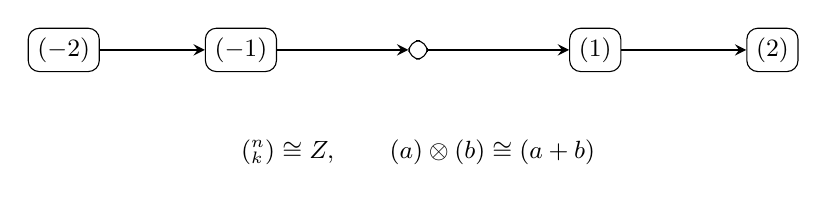
\begin{tikzpicture}[>=stealth,every node/.style={font=\small}]
\node[draw,rounded corners] (m2) at (-4.5,0) {$\OO(-2)$};
\node[draw,rounded corners] (m1) at (-2.25,0) {$\OO(-1)$};
\node[draw,rounded corners] (z) at (0,0) {$\OO$};
\node[draw,rounded corners] (p1) at (2.25,0) {$\OO(1)$};
\node[draw,rounded corners] (p2) at (4.5,0) {$\OO(2)$};
\draw[->,thick] (m2)--(m1);
\draw[->,thick] (m1)--(z);
\draw[->,thick] (z)--(p1);
\draw[->,thick] (p1)--(p2);
\node at (0,-1.3) {$\Pic(\PP^n_k)\cong\mathbb Z,\qquad \OO(a)\otimes\OO(b)\cong\OO(a+b)$};
\end{tikzpicture}
\caption{The twisting sheaves form the integer lattice of the Picard group of projective space, generated by \(\OO(1)\).}
\label{fig:vi42-projective-ladder}
\end{figure}
